\documentclass[Main.tex]{subfiles}
\begin{document}
\tableofcontents
\newpage	
\chapter{LME commands}

\texttt{vcov} returns the variance-covariance matrix of the main parameters of a fitted model object.
\begin{framed}
	\begin{verbatim}
> vcov(JS.roy1)
         methodJ  methodS
methodJ 11.01701  9.30105
methodS  9.30105 11.75301
\end{verbatim}
\end{framed}

\texttt{getVarCov} extract the variance-covariance matrix from a fitted model, such as a mixed-effects model.
\begin{framed}
\begin{verbatim}
> getVarCov(JS.roy1)
Random effects variance covariance matrix
        methodJ methodS
methodJ  923.98  785.23
methodS  785.23  971.29
Standard Deviations: 30.397 31.166 
\end{verbatim}
\end{framed}	
	
\chapter{Model Diagnostics for MCS}

%-------------------------------------------------------------------------%
\begin{abstract}
Model diagnostic techniques, well established for classical models, have since been adapted for use with linear mixed effects models. However, diagnostic techniques for LME models are inevitably more difficult to implement, due to the increased complexity. \\ \bigskip


\citet{schab} describes the examination of model-data agreement as comprising several elements; \begin{itemize}
		\item residual analysis, 
		\item goodness of fit, 
		\item collinearity diagnostics
		\item influence analysis.
	\end{itemize} 
	
This chapter is comprised of two sections:
\begin{enumerate}
	\item Residual Diagnostics
	\item Influence Diagnostics
\end{enumerate}
\end{abstract}

%=============================================================================== %
\newpage
\section{Introduction}
In statistical modelling, the process of model validation is a critical step, but also a step that is too often overlooked. A very simple procedure is to examine well known
metrics, such as the AIC and $R^2$ measures. However, using a small handful of simple measures and methods is insufficient to properly assess the quality of a fitted model. To do so properly, a full and comprehensive
analysis that tests of all of the assumptions, as far as possible, must be carried out. 

A statistical model, whether of the fixed-effects or mixed-effects variety, represents how you think your data were generated. Following model specification and estimation, it is of interest to explore the model-data
agreement by raising pertinent questions. Further to the analysis of residuals, \citet{schab} recommends the examination of the following questions.
\begin{itemize}
	\item Does the model-data agreement support the model assumptions?
	\item Should model components be refined, and if so, which components? For example, should certain explanatory variables
	be added or removed, and is the covariance of the observations properly specified?
	\item Are the results sensitive to model and/or data? Are individual data points or groups of cases particularly
	influential on the analysis?
\end{itemize}
\newpage
\section{Residual diagnostics} %1.3
\subsection{Introduction to Residual Analysis}
%A residual is the difference between an observed quantity and its estimated or predicted value. 
Residual analysis is a widely used model validation technique. A residual is simply the difference between an observed value and the corresponding fitted value, as predicted by the model. The rationale is that, if the model is properly fitted to the model, then the residuals would approximate the random errors that one should expect; if the residuals behave randomly, with no discernible trend. If some sort of non-random trend is evident in the model, then the model can be considered to be poorly fitted.

For classical linear models, residual diagnostics are typically implemented as a plot of the observed residuals and the predicted values. A visual inspection for the presence of trends inform the analyst on the validity of distributional assumptions, and to detect outliers and influential observations. Statistical software environments, such as the \texttt{R} programming language, provides a suite of tests and graphical procedures for appraising a fitted linear model, with several 
of these procedures analysing the model residuals.

However, for LME models the matter of residual is more complex, both from a theoretical point of view and from the practical matter of implementing a comprehensive analysis using statistical software. As the LME model can be tailored to the needs of the particular research question, the rationale behind the model appraisal must follow accordingly.


%===================================================================================================%
\subsection{Residuals in the Blood Data Example}
The fitted model used in the Blood data example, \texttt{JS.roy1}, was fitted using the \texttt{lme()} function from the nlme package, and as such, is stored as an \texttt{lme} object. The \texttt{residual} functions extracts residuals of a fitted LME model, depending on the type of residual required.

For an lme object, the residuals at level $i$ are obtained by subtracting the fitted levels at that level from the response vector (and dividing by the estimated within-group standard error, if \texttt{type="pearson"}).The Pearson residual is the raw residual divided by the square root of the variance function (here, the Within-group standard error for both methods, 6.11 and 9.11 respectively). The fitted values at level $i$ are obtained by adding together the population fitted values (based only on the fixed effects estimates) and the estimated contributions of the random effects to the fitted values at grouping levels less or equal to $i$.

\begin{description}
	\item["\texttt{response}"]: the “raw” residuals (\textit{observed - fitted}) are used. This is the default option.
	\item["\texttt{pearson}"]: the standardized residuals (raw residuals divided by the corresponding standard errors) are used; 
	\item["\texttt{normalized}"]: the normalized residuals (standardized residuals pre-multiplied by the inverse square-root factor of the estimated error correlation matrix) are used.
\end{description}

\begin{framed}
\begin{verbatim}
data.frame( response = resid(JS.roy1, type = "response"), 
            pearson  = resid(JS.roy1, type = "pearson"), 
          normalized = resid(JS.roy1, type = "normalized") )
\end{verbatim}
\end{framed}

\begin{verbatim}
                response      pearson    normalized
        1    -4.65805902 -0.761587227 -0.7615872269
        2    -0.88701342 -0.145025661  0.0776238081
        3    -5.16580898 -0.844603753 -0.8446037530
        4     2.29041830  0.374480726  0.6450898404
        5     7.87508366  1.287567009  1.2875670086
        6    -6.57048659 -1.074266908 -1.5090772378
        ...........................................
\end{verbatim}
For the $J$ observations, the variance is 6.116252 whereas for the $S$ observations, the denominator is 9.118144. (with the expected ratio of  1.490806)


\begin{framed}
\begin{verbatim}
> pearson %>%
+   as.numeric %>% 
+   matrix(nrow=85) %>%
+   round(4) 
                 [,1]    [,2]    [,3]    [,4]    [,5]    [,6]
         [1,] -0.7616  0.2194  0.3829 -0.2983  0.3597 -0.0790
         [2,] -0.1450  0.1820 -0.1450 -0.5014  0.1567  0.2663
         [3,] -0.8446  0.4634  0.1364 -0.1630 -0.2727  0.1660
         [4,]  0.3745 -0.2795 -0.2795 -0.2658 -0.2658  0.6115
         [5,]  1.2876 -0.6744 -0.6744  0.8935 -0.0935 -0.8612
         [6,] -1.0743  1.8687 -0.7473 -0.0383  0.2908 -0.3673
         ...........................................
         
\end{verbatim}
\end{framed}

We can plot the residuals against the fitted values, to assess the assumption of constant variance. 
\begin{framed}
\begin{verbatim}
# standardized residuals versus fitted values 
plot(JS.roy1, resid(., type = "pearson") ~ fitted(.) , 
    abline = 0, id = 0.05)
\end{verbatim}
\end{framed}
\begin{figure}[h!]
\centering
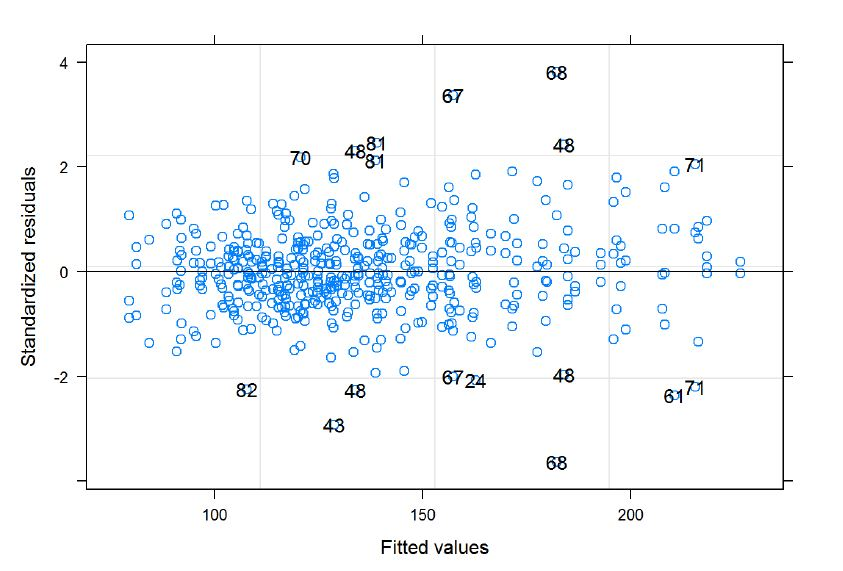
\includegraphics[width=0.9\linewidth]{Residuals-JS-Roy}
\caption{}
\label{fig:Residuals-JS-Roy}
\end{figure}

%===================================================================================================%
\subsection{Normality of Residuals in the Blood Data Example}
LME models assume that the residuals of the model are normally distributed.  The residuals can be divided according to groups according to the method of measurement. In the following examples, we seperately assess normality the \textit{J} method residuals (the first 255 residuals) and \textit{S} method residuals (the remaining 255). Importantly the residuals from the \textit{J} method are normally distributed, but there is non-normality of the residuals according to the \textit{S} method.
\begin{framed}
\begin{verbatim}
> shapiro.test(resid(JS.roy1)[1:255])

Shapiro-Wilk normality test

data:  resid(JS.roy1)[1:255]
W = 0.9931, p-value = 0.2852
\end{verbatim}
\end{framed}

\begin{framed}
	\begin{verbatim}
> shapiro.test(resid(JS.roy1)[256:510])

Shapiro-Wilk normality test

data:  resid(JS.roy1)[256:510]
W = 0.9395, p-value = 9.503e-09
\end{verbatim}
\end{framed}
\begin{figure}[h!]
\centering
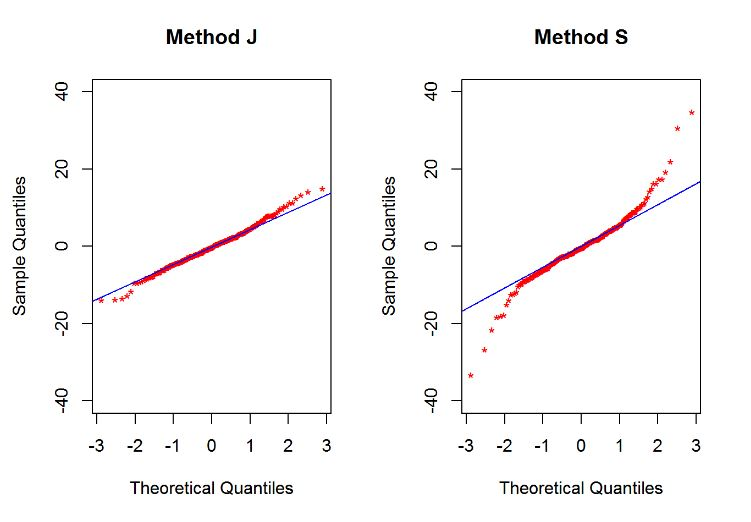
\includegraphics[width=0.9\linewidth]{Resid-newplot2}
\caption{}
\label{fig:Resid-newplot2}
\end{figure}

\newpage


\subsection{Conditional and Marginal Residuals}
A residual is the difference between an observed quantity and its estimated or predicted value. For LME models, \citet{schab} describes two types of residuals, marginal residuals and conditional residuals. 

\begin{itemize}
	\item A marginal residual is the difference between the observed data and the estimated (marginal) mean, $r_{mi} = y_i - x_0^{\prime} \hat{b}$
	\item A conditional residual is the difference between the observed data and the predicted value of the observation,
	$r_{ci} = y_i - x_i^{\prime} \hat{b} - z_i^{\prime} \hat{\gamma}$	
\end{itemize} 
In a model without random effects, both sets of
residuals coincide \citep{schab} . We shall revert to this matter in due course.



%\subsection{Marginal and Conditional Residuals}




In linear mixed effects models, diagnostic techniques may consider `conditional' residuals. A conditional residual is the difference between an observed value $y_{i}$ and the conditional predicted value $\hat{y}_{i} $.

\[ \hat{\epsilon}_{i} = y_{i} - \hat{y}_{i} = y_{i} - ( X_{i}\hat{\beta} + Z_{i}\hat{b}_{i}) \]

However, using conditional residuals for diagnostics presents difficulties, as they tend to be correlated and their variances may be different for different subgroups, which can lead to erroneous conclusions.
%========================================================%
\newpage
\subsection{Residual Analysis for MCS}

\begin{figure}[h!]
\centering
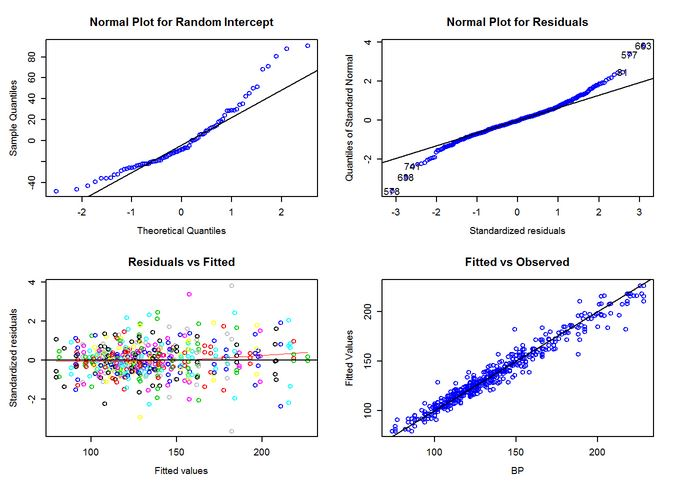
\includegraphics[width=0.9\linewidth]{ResidPlot}
\caption{}
\label{fig:ResidPlot}
\end{figure}

	%---------------------------------------------------------------------------%
\newpage
\section{Introduction to Influence analysis} %1.7
 Model diagnostic techniques determine whether or not the distributional assumptions are satisfied, and to assess the influence of unusual observations. In classical linear models model diagnostics have been become a required part of any statistical analysis, and the methods are commonly available in statistical packages and standard textbooks on applied regression. However it has been noted by several papers that model diagnostics do not often accompany LME model analyses.
For linear models for uncorrelated data, it is not necessary to refit the model after removing a data point in order to measure the impact of an observation on the model. The change in fixed effect estimates, residuals, residual sums of squares, and the variance-covariance matrix of the fixed effects can be computed based on the fit to the full data alone. By contrast, in mixed models several important complications arise. Data points can affect not only the fixed effects but also the covariance parameter estimates on which the fixed-effects estimates depend. 

\subsection{What is Influence} %1.1.5


Broadly defined, influence is understood as the ability of a single or multiple data points, through their presence or absence in the data, to alter important aspects of the analysis, yield qualitatively different inferences, or violate assumptions of the statistical model. The goal of influence analysis is not primarily to mark data points for deletion so that a better model fit can be achieved for the reduced data, although this might be a result of influence analysis \citep{schabenberger}.


\subsection{Importance of Influence}
The influence of an observation can be thought of in terms of how much the predicted values for other observations would differ if the observation in question were not included in the model fit.
Likelihood based estimation methods, such as ML and REML, are sensitive to unusual observations. Influence diagnostics are formal techniques that assess the influence of observations on parameter estimates for $\beta$ and $\theta$. A common technique is to refit the model with an observation or group of observations omitted. The basic procedure for quantifying influence is simple as follows:


\begin{enumerate}
	\item Fit the model to the data and obtain estimates of all parameters.
	\item Remove one or more data points from the analysis and compute updated estimates of model parameters.
	\item Based on full- and reduced-data estimates, contrast quantities of interest to determine how the absence of the observations changes the analysis.
\end{enumerate}
\subsection{Measures of Influence} 
% DFBETA
% DFFITS
% PRESS
The impact of an observation on a regression fitting can be determined by the difference between the estimated regression coefficient of a model with all observations and the estimated coefficient when the particular observation is deleted. DFBETA and DFFITS are well known measures of influenc. The measure DFBETA is the studentized value of this difference.	DFFITS is a statistical measured designed to a show how influential an observation is in a statistical model. DFFITS is closely related to the studentized residual.

\begin{eqnarray}
DFBETA_{a} &=& \hat{\beta} - \hat{\beta}_{(a)} \\
&=& B(Y-Y_{\bar{a}}
\\ DFFITS = {\widehat{y_i} -
	\widehat{y_{i(k)}} \over s_{(k)} \sqrt{h_{ii}}} 
\end{eqnarray}

The prediction residual sum of squares (PRESS) is an value associated with this calculation. When fitting linear models, PRESS can be used as a criterion for model selection, with smaller values indicating better model fits.
\begin{displaymath}
PRESS = \sum(y-y^{(k)})^2
\end{displaymath}
%	
%	\begin{itemize}
%		\item $e_{-Q} = y_{Q} - x_{Q}\hat{\beta}^{-Q}$
%		\item $PRESS_{(U)} = y_{i} - x\hat{\beta}_{(U)}$
%	\end{itemize}
%	
\subsection{DFBETAs}
The measure that measures how much impact each observation has on a particular predictor is DFBETAs The DFBETA for a predictor and for a particular observation is the difference between the regression coefficient calculated for all of the data and the regression coefficient calculated with the observation deleted, scaled by the standard error calculated with the observation deleted.

DFBETA is a measure found for each observation in a dataset. The DFBETA for a 
particular observation is the difference between the regression coefficient for an included variable calculated for all of the data and the regression coefficient calculated with the observation deleted, scaled by the standard error calculated with the 
observation deleted. 

The cut-off value for DFBETAs is $\frac{2}{\sqrt{n}}$, where n is the number of observations. 
However, another cut-off is to look for observations with a value greater than 1.00. Here cutoff means, 
“this observation could be overly influential on the estimated coefficient.” 
%==========================================================================%
%WIKIPEDIA
\subsubsection{DFFITS}
DFFITS is a diagnostic meant to show how influential a point is in a statistical regression. It was proposed in 1980. It is defined as the change ("DFFIT"), in the predicted value for a point, obtained when that point is left out of the regression, "Studentized" by dividing by the estimated standard deviation of the fit at that point:
\[ \mbox{DFFITS} = {\widehat{y_i} - \widehat{y_{i(i)}} \over s_{(i)} \sqrt{h_{ii}}}\]

\subsubsection{DFbetas for Blood Data}
\begin{framed}
	\begin{verbatim}
	plot(JS.roy1.dfbeta$all.res1[1:255],JS.roy1.dfbeta$all.res2[256:510],
	pch=16,col="blue")
	abline(v=JS.roy1.dfbeta$all.res1[256],col="red")
	abline(h=JS.roy1.dfbeta$all.res2[1],col="red")
	\end{verbatim}
\end{framed}
\begin{figure}
	\centering
	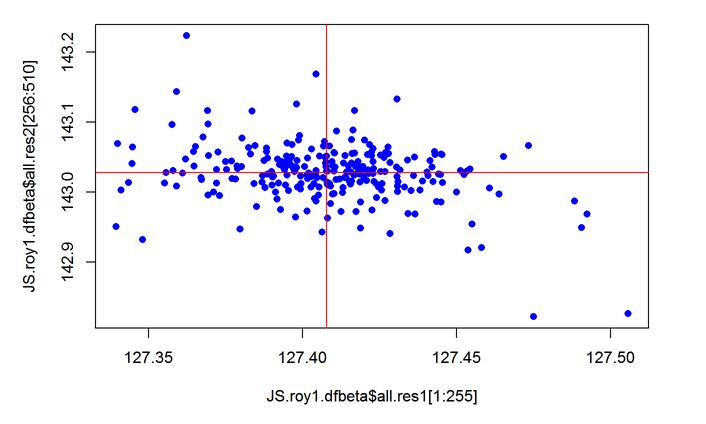
\includegraphics[width=0.7\linewidth]{dfbetas-JS-ROY}
	\caption{}
	\label{fig:dfbetas-JS-ROY}
\end{figure}


\section{Case Deletion Diagnostics}
Case-deletion diagnostics provide a useful tool for identifying influential observations and outliers.

The computation of case deletion diagnostics in the classical model is made simple by the fact that estimates of $\beta$ and $\sigma^2$, which exclude the ith observation, can be computed without re-fitting the model. Such update formulas are available in the mixed model only if you assume that the covariance parameters are not affected by the removal of the observation in question. This is rarely a reasonable assumption.

Linear models for uncorrelated data have well established measures to gauge the influence of one or more
observations on the analysis. For such models, closed-form update expressions allow efficient computations
without refitting the model. 


Since the pioneering work of Cook in 1977, deletion measures have been applied to many statistical models for identifying influential observations. Case-deletion diagnostics provide a useful tool for identifying influential observations and outliers.

The key to making deletion diagnostics useable is the development of efficient computational formulas, allowing one to obtain the \index{case deletion diagnostics} case deletion diagnostics by making use of basic building blocks, computed only once for the full model.

The computation of case deletion diagnostics in the classical model is made simple by the fact that estimates of $\beta$ and $\sigma^2$, which exclude the $i-$th observation, can be computed without re-fitting the model. %\subsection{Terminology for Case Deletion diagnostics} %1.8

\citet{preisser} describes two type of diagnostics. When the set consists of only one observation, the type is called
`\textit{observation-diagnostics}'. For multiple observations, Preisser describes the diagnostics as `\textit{cluster-deletion}' diagnostics. When applied to LME models, such update formulas are available only if one assumes that the covariance parameters are not affected by the removal of the observation in question. However, this is rarely a reasonable assumption.




%---------------------------------------------------------------------------%
%---------------------------------------------------------------------------%
\newpage
\subsection{Local Influence Analysis}



% - \citet{Beckman}
Beckman, Nachtsheim and Cook (1987)  applied the \index{local influence}local influence method of Cook (1986) to the analysis of the linear mixed model.

While the concept of influence analysis is straightforward, implementation in mixed models is more complex. Update formulae for fixed effects models are available only when the covariance parameters are assumed to be known.

If the global measure suggests that the points in $U$ are influential, the nature of that influence should be determined. In particular, the points in $U$ can affect the following

\begin{itemize}
	\item the estimates of fixed effects,
	\item the estimates of the precision of the fixed effects,
	\item the estimates of the covariance parameters,
	\item the estimates of the precision of the covariance parameters,
	\item fitted and predicted values.
\end{itemize}


\newpage
\subsection{Likelihood Distances}

The \index{likelihood distance} likelihood distance is a global summary measure that expresses the joint influence of the subsets of observations, $U$, on all parameters in $\phi$ that were subject to updating. For classical linear models, the implementation of influence analysis is straightforward. \citet{schab} points out the likelihood distance gives the amount by which the log-likelihood of the model fitted from the full data changes if one were
to estimate the model from a reduced-data estimates. Importantly $LD(\psi_{(U)})$ is not the log-likelihood obtained by fitting the model to the reduced data set. It is obtained by evaluating the likelihood function based on the full data set (containing all $n$ observations) at the reduced-data estimates.


%---------------------------------------------------------- %
%Likelihood Displacement.
\[  LD(\boldsymbol{(U)})= 2[l\boldsymbol{\hat{(\phi)}} - l\boldsymbol{\hat{\phi}_\omega} ] \]
\[  RLD(\boldsymbol{(U)})= 2[ l_R\boldsymbol{\hat{(\phi)}} - l_R\boldsymbol{\hat{(\phi)}_\omega} ] \]
%	Large values indicate that $\boldsymbol{\hat{\theta}}$ and $\boldsymbol{\hat{\theta}_\omega}$ differ considerably.


An overall influence statistic measures the change in the objective function being minimized. For example, in
OLS regression, the residual sums of squares serves that purpose. In linear mixed models fit by
\index{maximum likelihood} maximum likelihood (ML) or \index{restricted maximum likelihood} restricted maximum likelihood (REML), an overall influence measure is the \index{likelihood distance} likelihood distance \citep{cook}. In LME models, fitted by either ML or REML, an important overall
 influence measure is the likelihood distance \citep{cook82}. The  procedure requires the calculation of the full data estimates
 $\hat{\psi}$ and estimates based on the reduced data set  $\hat{\psi}_{(U)}$. The likelihood distance is given by
 determining
 
 
 \begin{eqnarray}
 LD_{(U)} &=& 2\{l(\hat{\psi}) - l( \hat{\psi}_{(U)}) \}\\
 RLD_{(U)} &=& 2\{l_{R}(\hat{\psi}) - l_{R}(\hat{\psi}_{(U)})\}
 \end{eqnarray}
%----schabenberger page 8
For classical linear models, the implementation of influence analysis is straightforward.
However, for LME models, the problem is more complex. Update formulas for the fixed effects are available only when the covariance parameters are assumed to be known. A measure of total influence requires updates of all model parameters. This can only be achieved in general is by omitting observations or cases, then refitting the model. This is a very simplistic approach, and computationally expensive.

\citet{west} examines a group of methods that examine various aspects of influence diagnostics for LME models.
For overall influence, the most common approaches are the \textit{likelihood distance} and the \textit{restricted likelihood distance}.

\subsubsection{The \texttt{logLik} Function}
\texttt{logLik.lme} returns the log-likelihood value of the linear mixed-effects model represented by object evaluated at the estimated coefficients. It is also possible to determine the restricted log-likelihood, if relevant, using this function. For the Blood Data Example,  the loglikelihood of the JS.roy1 model can be computed as follows.
\begin{framed}
\begin{verbatim}
> logLik(JS.roy1)
'log Lik.' -2030.736 (df=8)
\end{verbatim}
\end{framed}
%======================================================================================= %
\newpage
\subsection{Cook's Distance}
\citet{CPJ} develops \index{case deletion diagnostics} case deletion diagnostics, in particular the equivalent of \index{Cook's distance} Cook's distance, a well-known metric, for diagnosing influential observations when estimating the fixed effect parameters and variance components. Deletion diagnostics provide a means of assessing the influence of an observation (or groups of observations) on inference on the estimated parameters of LME models. 
%We shall provide a fuller discussion of Cook's distance in due course.
Cook's Distance is a good measure of the influence of an observation that is a measure of aggregate impact of each observation on the group of regression coefficients, as well as the group of fitted values.
%Cook's Distance is proportional to the sum of the squared differences between predictions made with all observations in the analysis and predictions made leaving out the observation in question. 
If the predictions are the same with or without the observation in question, then the observation has no influence on the regression model. If the predictions differ greatly when the observation is not included in the analysis, then the observation is influential.

%======================================================================================= %
\newpage
% Hence the name deletion diagnostics and case-deletion diagnostics. 
\subsubsection{Cook's Distance for Blood Data}
\begin{figure}[h!]
	\centering
	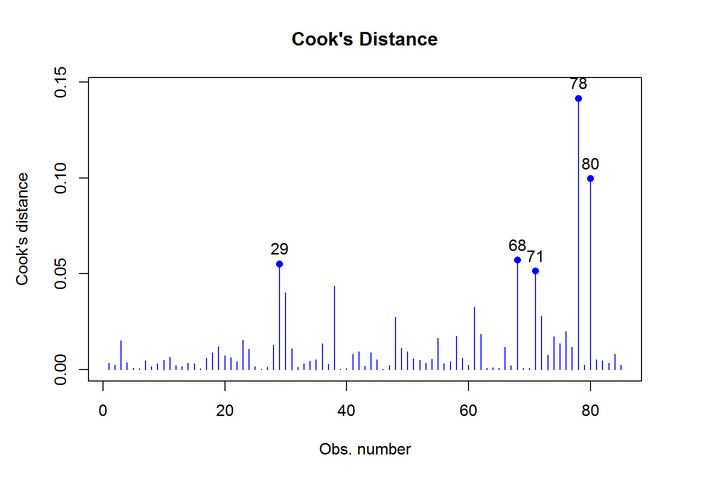
\includegraphics[width=0.9\linewidth]{CooksDistancePlot-JS-Roy}
	\caption{}
	\label{fig:CooksDistancePlot-JS-Roy}
\end{figure}

\newpage



\bibliography{DB-txfrbib}
\end{document}
%================================================================================ %